%!TEX root = origin_elements_lecture_notes.tex

\chapter{The Fate of Massive Stars}\label{ch:massive_stars}
Compared to stars with masses of up to $\sim 8\,M_\odot$, massive stars undergo different burning phases that significantly differ from what was discussed in Chapter~\ref{ch:sun}. Here, we will first discuss observations that led to the discovery and classification of massive stars and their properties. We will then discuss in more details how massive stars evolve and ultimately die before discussing massive star contributions of freshly nucleosynthesized material to the solar nebula 4.5\,Ga ago.

\section{Observations}

\subsection{Wolf-Rayet Stars} In 1867, the French astronomers Charles Wolf and Georges Rayet observed three stars in the Cygnus constellation that emitted unusually broad emission instead of the typical absorption lines. Along with these emission lines, these now so-called \ac{wr} stars are also very hot with effective temperatures of $(25 - 100)\times 10^{3}$\,K. \ac{wr} stars also show very high mass losses in excess of $10^{-5}\,M_\odot$\,a$^{-1}$ with wind speeds ranging from 800\,km\,s$^{-1}$ to 3000\,km\,s$^{-1}$ and many are rapidly rotating with typical equatorial speeds of around 300\,km\,s$^{-1}$. Figure~\ref{fig:massive_stars:wr124} shows an image of a \ac{wr} star, namely star WR124. 

In addition, the spectra different \ac{wr} show different compositions. The spectra of WN stars are dominated by emission lines of helium and nitrogen. For WC stars, helium and carbon dominate the spectra while nitrogen and hydrogen are absent. Finally, WO stars, which are rarer than the other two types, contain prominent oxygen lines and have some contribution to their spectra from highly ionized species. These different features are direct consequences of the mass loss of these massive stars.


\subsection{Supernovae}
\begin{figure}[tb]
    \centering
    \begin{subfigure}{0.495\textwidth}
        \includegraphics[width=\textwidth]{graphics/massive_stars/wr124}
        \caption{Wolf-Rayet star WR124. Credit: ESA, Hubble \& NASA.}
        \label{fig:massive_stars:wr124}
    \end{subfigure}
    \begin{subfigure}{0.495\textwidth}
        \includegraphics[width=\textwidth]{graphics/massive_stars/crab_nebula}
        \caption{The crab nebula. Credit: NASA, ESA, NRAO/AUI/NSF \& G. Dubner.}
        \label{fig:massive_stars:crab_nebula}
    \end{subfigure}
    \caption{Massive stars at different evolutionary times.}
    \label{fig:massive_stars:massive_stars_figure}
\end{figure}
Throughout the written history of humanity, new stars have been observed all over the world. Based on various writings from astrologers in China, Egypt, Europe, Iraq, and Japan, a star appeared in the Taurus constellation around April 30, 1006, and faded from view about one year later. Modern telescopes allowed the detection of the remnant of this new star which can today still be detected as the crab nebula. This \ac{sn} remnant is shown in Figure~\ref{fig:massive_stars:crab_nebula}. While the last \ac{sn} to occur in the Milky Way was in 1604, an event that was reported by Tycho Brahe and Johannes Kepler, supernovae in other galaxies can also be observed with modern telescopes. 

One event that deserves special mentioning is \ac{sn} 1987A. Since multiple \acp{sn} are recorded every year, they are now cataloged with the year and a subsequent letter. \ac{sn} 1987A was discovered on February 24, 1987, in the large Magellanic cloud, a satellite galaxy of the Milky Way. It was quickly determined that the progenitor of this event was a blue supergiant star. The proximity of the event further allowed it to be studied with various techniques. For example, the light curve could be measured and analyzed in detail. Furthermore, a total of 20 neutrinos from \ac{sn} 1987A were detected in Japan and the US. These neutrinos arrived three hours before the photons of the event reached Earth, thus significantly constraining the upper limit of the neutrino mass.

\begin{figure}[tb]
    \centering
    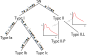
\includegraphics[width=0.6\textwidth]{graphics/massive_stars/sn_classification}
    \caption{Classifaction of \acp{sn} based on their spectra at maximum light and their light curves.}
    \label{fig:massive_stars:sne_classification}
\end{figure}
Figure~\ref{fig:massive_stars:sne_classification} shows a schematic on how supernovae are classified based on observational properties. Note that this classification is purely based on (1) the spectral lines present and (2) the shape of the light curve. If no hydrogen lines are present in \ac{sn} it is classified as a type I \acl{sn}, otherwise as an \ac{snii}. Type I \acp{sn} are further subdivided into three categories: \ac{snia} contain no singly-ionized silicon (Si II) lines while \ac{snib} and \ac{snic} do. The former in additional show helium lines while the latter do not. If the spectrum of the \ac{sn} shows hydrogen lines, it is by definition a \ac{snii}. Further subdivisions are based on the light curve emitted by the event. Figure~\ref{fig:massive_stars:sne_classification} shows examples of light curves. If it contains a plateau it is called a \ac{sniip}, otherwise an \ac{sniil}. We will see later why the different types show the specific features mentioned in Figure~\ref{fig:massive_stars:sne_classification}.



\section{The Evolution of Massive Stars}

Before we discuss in detail how \acp{sn} explode, let us discuss the individual burning phases that stars with masses $M \gtrsim 8\,M_\odot$ undergo.
\begin{figure}[tb]
    \centering
    \includegraphics[width=0.8\textwidth]{graphics/massive_stars/hrd_massive_stars}
    \caption{Evolution of various massive stars in the \ac{hrd} after they left the main sequence. Data from \citet{pignatari16}.}
    \label{fig:massive_stars:hrds_pignatari_nugrid_set1.2}
\end{figure}
Figure~\ref{fig:massive_stars:hrds_pignatari_nugrid_set1.2} shows the evolution of massive stars in the \ac{hrd}. Stellar models are for a metallicity of $Z=0.02$ and are taken from \citet{pignatari16}. The paths of the stars on the \ac{hrd} start when they leave the main sequence. While the evolution of the shown stars all look fairly similar, they are vastly different from the fate that lower-mass stars undergo. Here, the $25\,M_\odot$ star is discussed as an example. Such a star lives for around 9\,Ma \citep{meynet03}. Even though massive stars are much rarer than low-mass stars, the short lifetime results in these stars rapidly recycling freshly nucleosynthesized material back into the Milky Way, thus enriching it in metallicity. Recycling also takes place prior to the supernova, since stellar winds can drive parts of the atmosphere out into space. 

\begin{table}[b]\label{codebox:nugrid}
\codebox{NuGrid Collaboration and Data Access}{The \href{https://nugrid.github.io/}{Nucleosynthesis Grid (NuGrid) international collaboration} develops and maintains tools for large-scale nucleosynthesis post-processing simulations and to analyze stellar evolution models created with MESA. Especially interesting is that all stellar models and postprocessing data is released publicly. NuGrid maintains a public JupyterLab server that can be accessed by anybody to explore stars. This systems has also been used to create Figure~\ref{fig:massive_stars:hrds_pignatari_nugrid_set1.2} and is available on the \href{https://astrohub.uvic.ca/}{University of Victoria's AstroHub site}.}
\end{table}

\paragraph{Helium burning}
Hydrogen burning takes place for around 90\% of the star's lifetime, mainly via the CNO cycle (see Figure~\ref{fig:sun:energy_generation_hydrogen_fusion}). When the core is exhausted, hydrogen burning continues in a shell. The core starts contracting until the temperature is high enough to ignite helium burning, at which point the star significantly increases in size and becomes a supergiant. Examples of such stars are Rigel or Betelgeuse, a blue and red supergiant, respectively, in the constellation Orion. In fact, on a clear night in winter you can easily identify these two stars by eye due to their color. Helium burning in the core lasts for less than 1\,Ma and during this time, neutron captures can lead to the formation of some heavy nuclei with $A>60$. This is the so-called weak \ac{sproc} and is responsible for the \ac{sproc} isotopes between nickel and strontium. Details on the \ac{sproc} will be discussed in Chapter~\ref{ch:s-process}. 

\paragraph{Carbon, neon, and oxygen burning}
The ashes left behind after helium burning mainly consist of \ex{12}C and \ex{16}O. Of the possible reactions, carbon burning has the lowest threshold and starts first. The main reactions are as already seen in~\eqref{eqn:sun:carbon_burning_reactions}.
The main leftovers after this reaction are \ex{16}O and \ex{20}Ne.

After carbon burning, the star contracts once more and the temperature and density rise to a point at which photodisintegration reactions become important. This in fact first leads to the reaction
\begin{equation}
    {^{20}}\mathrm{Ne} + \gamma \longrightarrow {^{16}}\mathrm{O} + \alpha,
\end{equation}
which is endothermic and consumes 4.73\,MeV of energy. Note that $\alpha$ is equivalent to a \ex{4}He nucleus. Subsequent, main exothermic reactions that take place during neon burning are
\begin{align}
    {^{20}}\mathrm{Ne} + \alpha &\longrightarrow {^{24}}\mathrm{Mg} + \gamma \\
    {^{24}}\mathrm{Mg} + \alpha &\longrightarrow {^{28}}\mathrm{Si} + \gamma \\
    {^{23}}\mathrm{Na} + \alpha &\longrightarrow {^{26}}\mathrm{Mg} + p \\
    {^{26}}\mathrm{Mg} + \alpha &\longrightarrow {^{29}}\mathrm{Si} + n.
\end{align}
Here, $p$ stands for an individual proton. The overarching production taking place during neon burning is
\begin{equation}
    {^{20}}\mathrm{Ne} + {^{20}}\mathrm{Ne} \longrightarrow {^{16}}\mathrm{O} + {^{24}}\mathrm{Mg}
\end{equation}
and releases 4.6\,MeV of energy.

After neon has efficiently been destroyed, \ex{16}O, \ex{24}Mg, and \ex{28}Si are the most abundant nuclei in the star. Again the core contracts and heats up until oxygen burning starts. The important reactions are:
\begin{equation}
{^{16}}\mathrm{O} + {^{16}}\mathrm{O} \longrightarrow 
    \begin{cases}
        {^{24}}\mathrm{Mg} + 2\,{^4}\mathrm{He} \quad & (*)\\
        {^{28}}\mathrm{Si} + {^4}\mathrm{He}\\
        {^{30}}\mathrm{P} + d \quad & (*)\\
        {^{31}}\mathrm{P} + p\\
        {^{30}}\mathrm{S} + 2\,p\\
        {^{31}}\mathrm{S} + n\\
        {^{32}}\mathrm{S} + \gamma
    \end{cases}
    \label{eqn:massive_stars:oxygen_burning_reactions}
\end{equation}
Here $d$ stands for a deuterium nucleus. 

\paragraph{Silicon burning}
At the end of oxygen burning, the most abundant nuclei in the star are \ex{28}Si and \ex{32}S. The core again contracts, however, reactions combining \ex{28}Si and \ex{32}S directly are too unlikely to occur due to coulomb barrier considerations. Instead, the higher temperatures allow photodisintegration of some nuclei to form protons, neutrons, and \ex{4}He particles. These can subsequently be caught on \ex{28}Si and \ex{32}S to form heavier, more tightly bound nuclei. Silicon burning reactions take place on a timescale of about 1\,d and at temperatures in the range of $3-4$\,GK.

\begin{figure}[tb]
    \centering
    
\includegraphics[width=0.6\textwidth]{graphics/massive_stars/pre-supernova}
    \caption{Schematic structure of the pre-supernova star, not to scale. In black inidcated are the most abundant isotopes in each shell \citep{limongi2000}. Inidcated in red are the nuclear burning shells.}
    \label{fig:massive_stars:pre-supernova_structure_schematic}
\end{figure}
Figure~\ref{fig:massive_stars:pre-supernova_structure_schematic} shows a schematic of the star's composition at towards the end of the silicon burning. The inner core consists mostly of \ex{56}Fe and \ex{52}Cr. This onion like structure has lighter elements towards the surface and all composition changes are separated from each other by respective burning shells. Note that ashes of these nuclear fires accumulate at the bottom of each shell and get added to the inner parts, e.g., silicon burning is constantly adding ashes to the core.

\infobox{Coulomb barrier}{Since atomic nuclei are positively charged, they repell each other. The Coulomb barrier describes the energy that needs to be overcome in order for two nuclei to interact. With the nuclei at distance $r$ and charges $q_1$ and $q_2$, the Coulomb energy can be written as
\begin{equation}
    E_\mathrm{coul} = k_C \frac{q_1 q_2}{r}. \label{eqn:massive_stars:coulomb_energy}
\end{equation}
Here, $k_C=8.9876\times10^{9}$\,N\,m$^{2}$\,C$^{-2}$ is Coulomb's constant. 

\href{https://en.wikipedia.org/wiki/Quantum_tunnelling}{Quantum tunneling} enables two nuclei to fuse even below this energy. The conditions under which tunneling is allowed are found in the so-called \href{https://en.wikipedia.org/wiki/Gamow_factor}{Gamow window.}}

\paragraph{Nuclear statistical equilibrium}
At the end of silicon burning, once most of the \ex{28}Si has been processed further, the temperature and density in the star steadily increases until the point is reached at which production and destruction processes of nuclei come into equilibrium. Once every nuclei in the network from protons, neutrons, and \ex{4}He up to the iron peak nuclei is equally likely to be produced and destroyed, \ac{nse} is achieved. This will soon become more important, namely once the stellar explosion sets in.


\section{Core-Collapse Supernovae}

Depending on the initial mass of the star, various fates can yield a supernova explosion. In our example $25\,M_\odot$ case, the degenerate iron core of the pre-supernova (Figure~\ref{fig:massive_stars:pre-supernova_structure_schematic}) is constantly being fed with ashes from the silicon burning shell around it. Once the core mass reaches the \href{https://en.wikipedia.org/wiki/Chandrasekhar_limit}{Chandrasekhar limit} of roughly $1.4\,M_\odot$, the degeneracy pressure can no longer counteract the gravitational force and thus the core collapses freely with a speed of about $0.25c$. The core collapses to a density of $\rho\approx10^{14}$\,g\,cm$^{-3}$, which is similar to the density of the nuclei themselves. At this point, the strong force, which is usually attractive, becomes repulsive. Overshooting in nuclear density, the inner core of the star now acts as a stiff spring, which results in the creation of a shock wave and a bounce back that now travels outwards and passes the material form outer shells that is gravitationally collapsing onto the core. 

The outward moving shock leads to photodisintegrations of iron-peak nuclei, which in return removes energy from the shock wave itself. Further energy is lost by neutrino emission, which ultimately results in the shock stalling when it has reached the outer edge of the core around 1\,s after core collapse (10\,ms after the bounce). Infalling material now accretes onto the shock wave.

It is not yet clear how exactly the shock wave starts up again. One possibility is that a neutrinosphere builds up in the core from the processes of photodisintegration and electron capture. The area where the shock stalled is now so dense that neutrinos cannot easily penetrate it. Thus, these neutrinos are estimated to deposit around 5\% of their total energy in the matter just behind the shock. The heat deposited in this area allows the shock to be revived and continue its path towards the stellar surface. If this process does not occur, the material will fall back onto the core and ultimately lead to the formation of a neutron star or black hole, and no stellar explosion occurs. It is in fact still unclear what stars explode (mass, metallicity) and how exactly. Large supercomputers are being used to track the evolution of supernovae, however, due to the timescales and complexity of the problem, detailed 3D simulations progress slowly.\footnote{Some links to go down the rabbit hole: \href{https://ccsweb.lanl.gov/astro/index.html}{Center for Theoretical Astrophysics at Los Alamos National Laboratory}, \href{https://www.scidac.gov/}{Scientific Discovery through Advanced Computing (SciDAC)}, \href{https://2sn.org/}{Alex Heger}}

It is thought that \acp{snib}, \acp{snic}, and \acp{snii} are all result from core-collapse of a massive star. Differences originate from the original composition of the star, which also influences the exact mechanism of the supernova trigger.

\subsection{Explosive burning and freeze-out}

We have established the conditions for nuclear statistical equilibrium above, which is achieved at high enough temperatures. The shock wave, however, heats material as it travels outwards and thus induces further burning of these fuels in a process called explosive burning. As the shock moves outwards, the star expands and cools, thus material on the inside experiences a rapid decrease in temperature. 

Nucleosynthesis reactions taking place under these circumstances are highly dependent on the densities of free, light particles such as protons, neutrons, and $\alpha$-particles. If the fraction of available \ex{4}He nuclei is small, $\alpha$-poor freeze out takes place, resulting in the production of mostly iron peak elements such as \ex{56}Ni, \ex{54}Fe, and \ex{56}Fe. On the other hand, if many free $\alpha$-particles are available, $\alpha$-rich freeze out takes place, which creates elements along the chain of multiples of $\alpha$-particles, e.g., 
\begin{equation}
    \alpha (2\alpha, \gamma) ^{12}\mathrm{C} (\alpha, \gamma) ^{16}\mathrm{O} \quad \dots \quad ^{52}\mathrm{Fe} (\alpha, \gamma) ^{56}\mathrm{Ni}.
\end{equation}

\begin{figure}[tb]
    \centering
    
\includegraphics[width=0.6\textwidth]{graphics/massive_stars/post-supernova}
    \caption{Schematic structure of the post-supernova star, not to scale. Given are the 1-2 most abundant elements in every zone, which give the zone its name \citep{meyer95}. The gray area represents the material left behind in the explosion, either a neutron star or a black hole.}
    \label{fig:massive_stars:post-supernova_structure_schematic}
\end{figure}
Figure~\ref{fig:massive_stars:post-supernova_structure_schematic} shows the composition of the ejecta from a star post-supernova. Labels represent the most abundant element(s) for a given layer. These layers are generally named after the two most abundant elements present in them \citep{meyer95}.

\subsection{Fall-back}

Depending on the initial conditions of a star, e.g., mass and metallicity, either a neutron star or a black hole are left behind after the supernova explosions. Some of the material that first expands will get pulled back and fall onto the remnant. How much mass exactly falls back \citep[e.g.,][]{heger03} will define the amount of material that gets recycled back into the galaxy and thus contributes to its enrichment in metals.



\subsection{Neutrinos and Supernova Luminosity}

Assuming that the shock wave propagates through the star as discussed above, the total kinetic energy released in a supernova explosion is around $10^{44}$\,J. This is equivalent to roughly 1\% of the total energy released by neutrinos.

In both scenarios above, freeze-out conditions result in the production of \ex{56}Ni, a radioactive isotope of nickel. It decays to \ex{56}Co with a half-life of around 6\,d, which then furthermore decays to \ex{56}Fe with a half-life of 77.2\,d. Energy from the $\gamma$-rays that are emitted by the decaying nuclei is subsequently deposited into the thick, expanding envelope that moves away from the star. This envelope then radiates the energy in the form of visible light. The light curves of supernovae are thus determined by the radioactive decay taking place. The peak luminosity that is generally achieved is around $10^9\,L_\odot$, which is bright enough to outshine whole galaxies and thus explain the terminology: \acl{sn}. 

The plateau in \acp{sniip} (see inset in Figure~\ref{fig:massive_stars:sne_classification}) is likely the result of the recombination of hydrogen molecules, which emits light as the ejecta cools. Much less hydrogen is present in the envelopes of \acp{sniil}, thus no plateau in the light curve occurs.


\infobox{1\,foe}{Traditionally, the \ac{sn} community uses cgs units. The kinetic energy of a typical \ac{sn} shockwave in cgs units is around $10^{51}$\,erg. Gerald E. Brown and Hans Bethe coined the term 1\,foe, where foe stands for fifty-one erg, in order to have a more convenient way of talking about \acp{sn} explosions. Later, Steven Weinberg proposed to rename it to 1\,bethe (B). All notations are found in the literature.}



\section{Type Ia Supernovae}\label{sec:massive_stars:snia}

In contrast to core-collapse \acp{sn} described above, \ac{snia} take place in binary star systems. One remarkable property of these events is that their maximum luminosity seems to be very constant and only shows minor spread. Therefore, \acp{snia} are used as standard candles in cosmology, i.e., to determine distance to far away galaxy and to measure the Hubble constant and expansion rate of the universe. However, significant discrepancies have been found when determining the Hubble constant using \ac{snia} as standard candles and when measuring it via the \ac{cmb}.\footnote{\url{https://www.sciencenews.org/article/debate-universe-expansion-rate-hubble-constant-physics-crisis}} Recently, \citet{freedman19} used the brightness of stars on the tip of the red giant branch to determine the Hubble constant again. The result landed right in between the determination via \acp{snia} and using the \ac{cmb}. 

Aside from their effect on cosmology, \acp{snia} are also expected to contribute a significant amount of nucleosynthesized material to the Milky Way. A better understanding of their origin is thus crucial to decipher \ac{gce} as well as the cosmological implications.


\subsection{The Single-Degenerate Scenario}

The exact mechanisms behind \acp{snia} are poorly understood, however, researchers are focusing in on roughly two scenarios, both of which could occur in nature.
\begin{figure}[tb]
    \centering
    \includegraphics[width=0.75\textwidth]{graphics/massive_stars/sn-ia-artistic}
    \caption{Artistic view of the accretion that leads to a \ac{snia} explosion. Credit: NASA/JPL.}
    \label{fig:massive_stars:sn_ia_artistic}
\end{figure}
Figure~\ref{fig:massive_stars:sn_ia_artistic} shows an artistic view of the single-degenerate scenario for \ac{snia} explosions. In this scenario, a degenerate CO \ac{wd} accretes matter from a companion star at a relatively large rate of around $10^{-7}\,M_\odot\,\mathrm{a}^{-1}$. The companion star could, e.g., be a Red Giant. When the mass of the degenerate, primary star exceeds the Chandrasekhar limit ($\sim1.4\,M_\odot$), the carbon core ignites under degenerate conditions. A thermonuclear runaway occurs, which ultimately leads to the \ac{sn} explosion that completely disrupts the \ac{wd}. The companion star likely survives the explosion. During this explosion, nucleosynthesis takes place via nuclear statistical equilibrium, resulting in the production of mainly around $0.6\,M_\odot$ of \ex{56}Ni and some lighter nuclei. The amount of \ex{56}Ni is responsible for the typical and constant light curve.


\subsection{The Double-Degenerate Scenario}

In this scenario, the \ac{snia} occurs via the collision of \acp{wd}. In a close binary system, two \acp{wd} will spiral inwards because of momentum loss due to gravitational wave emission. Once close enough, the less massive star will start loosing mass to the more massive star. Once the mass of the degenerate core again reaches the Chandrasekhar limit, carbon burning ignites and proceeds similar to the single-degenerate scenario. In this case, both stars are completely disrupted leaving behind no remnant.


\subsection{Open Questions and the Cosmological ``Crisis''}

Many open questions remain with respect to \acp{snia}. It is unclear which scenario in fact leads to the formation of \acp{snia} and it could easily be the case that more than one trigger exists. Furthermore, metallicity likely has some influence on the exact explosion mechanism and on the light curve. One speculation to resolve the Hubble constant crisis is that \ac{snia} formation is different in galaxies at high redshifts compared to the near universe. This could potentially resolve the discrepancies without requiring ``new physics'' (see also Chapter~\ref{ch:bbn}). The recent measurements by \citet{freedman19} are surely a promising indication into this direction.



\section{Massive Star Contributions to the Early Solar System}

It has been shown \citep{jacobsen08} that the Solar System started with a canonical \ex{26}Al/\ex{27}Al ratio of $5\times10^{-5}$. Since \ex{26}Al is \iac{slr} with a half-life of $7.17\times10^{5}$\,a and decays to \ex{26}Mg. This \ac{slr} must have been supplied to the solar nebula shortly before the collapse of the molecular cloud and the subsequent formation of the first solids. 

\subsection{Isochron Measurements}

In order to determine the amount of \acp{slr} in meteoritic material, mineral phases with various different elemental aluminum-to-magnesium ratios are measured for their magnesium isotopic content. 
\begin{figure}[tb]
    \centering
    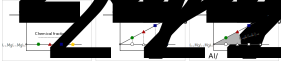
\includegraphics[width=\textwidth]{graphics/massive_stars/al26_isochron}
    \caption{Schematic representation to show how an isochron develops over time in different minerals within a given meteorite.}
    \label{fig:massive_stars:al26_isochron}
\end{figure}
Figure~\ref{fig:massive_stars:al26_isochron} shows a schematic of the formation for an isochron. Different mineral phases of a given meteorite (left) will incorporate various amounts of magnesium and aluminum according to their respective composition. If a phase incorporates live \ex{26}Al, the amount it incorporates is constant with respect to the amount of the stable \ex{27}Al. Over time, all \ex{26}Al decays, thus raising the respective \ex{26}Mg/\ex{24}Mg isotope ratio in the given phase (center panel in Figure~\ref{fig:massive_stars:al26_isochron}). Finally, when measured in a meteorite 4.567\,Ga later, measurements plotting on an isochron (right panel in Figure~\ref{fig:massive_stars:al26_isochron}) indicate a common age and can be used to derive the solids initial \ex{26}Al/\ex{27}Al ratio. Mathematically this can be expressed as
\begin{equation}
    \frac{^{26}\mathrm{Mg}}{^{24}\mathrm{Mg}} = \left(\frac{^{26}\mathrm{Al}}{^{27}\mathrm{Al}}\right)_0 \times \frac{^{27}\mathrm{Al}}{^{24}\mathrm{Mg}} + \left(\frac{^{26}\mathrm{Mg}}{^{24}\mathrm{Mg}}\right)_0.
\end{equation}
The slope of the linear correlation represents the wanted quantity; the initial \ex{26}Al/\ex{27}Al composition.


\subsection{The Iron-60 Controversy}

Using various mineral phases and in situ measurements of meteoritic phases, the initial composition of \ex{60}Fe/\ex{56}Fe was determined by various authors to be on the order of $10^{-7}$ to $10^{-6}$ \citep[e.g.,][]{mishra14,telus18}. This high abundance would be consistent with a co-production of \ex{26}Al and \ex{60}Fe in a \ac{sn}, which could also have triggered the collapse of the Solar System's molecular cloud.

On the other hand, bulk measurements of meteorites showed an initial \ex{60}Fe/\ex{56}Fe ratio for the early Solar System of $(1.01 \pm 0.27)\times10^{-8}$ \citep{tang12,tang15}. This \ex{60}Fe value could easily be consistent with the galactic background. More importantly it prohibits \acp{sn} from being the main contributor of \ex{26}Al. The longer life-time of \ex{60}Fe ($t_{\nicefrac{1}{2}} = 2.62 \times 10^{6}$\,a) with respect to \ex{26}Al only allows the \ex{26}Al/\ex{60}Fe ratio to decrease over time. Even within the uncertainties in the nucleosynthesis calculations, \acp{sn} would contribute too much \ex{60}Fe is supplying all \ex{26}Al \citep{jones19}. The origin of \ex{26}Al is thus likely a different stellar source, a likely candidate being nucleosynthesis in stellar winds of a \ac{wr} star \citep{dwarkadas17}.

The solution to the issue of measurement discrepancies likely originates in the data processing of the in situ measurements that determined the high \ex{60}Fe/\ex{56}Fe values. \citet{trappitsch18} re-measured one sample and found no effects due to in situ decay of \ex{60}Fe. These measurements and evaluations pointed into the direction of in situ data evaluation issues. Further work is currently ongoing and will likely solve the \ex{60}Fe controversy; no proof has so far been brought forward that the amount of \ex{60}Fe is different from what is expected from galactic background.


\section{Reading}

Please read \citet{fry15}. You may skim through Sections~3 and~4, however make sure you understand the ingredients for equation~(1). For discussion, focus on the big picture of what the authors are trying to address. Furthermore, many different fields play a role here. Try to decipher the connections and difficulties that the different researchers bump into when contributing to the big picture. The following points might help with the reading:

\begin{itemize}
    \item What isotope signatures have been found for a nearby, recent \ac{sn} explosion and where were these signals detected?
    \item How do the terrestrial and lunar records compare? What problems do you see with either record? What are advantages / disadvantages of one record over the other?
    \item What types of events could have contributed the \acp{slr}?
    \item Why are \ac{snia} and kilonovae ruled out as potential sources?
    \item Why is it important how much energy \acp{sn} deposit into the ejecta?
    \item Discuss the individual components that go into equation~(1). What issues do you see?
    \item Why are electron-capture supernovae the preferred explanation according to \citet{fry15} for the \ac{slr} record?
\end{itemize}
